\documentclass[12pt,a4paper]{article}

% ─── Page Layout ───────────────────────────────────────────────────────────────
\usepackage[a4paper, margin=0.8in, headheight=14pt]{geometry}

% ─── Fonts (XeLaTeX) ───────────────────────────────────────────────────────────
\usepackage{fontspec}
\usepackage{unicode-math}
\setmainfont{TeX Gyre Pagella}
\setmonofont[Scale=0.88]{TeX Gyre Cursor}
\setmathfont{Latin Modern Math}

% ─── Packages ──────────────────────────────────────────────────────────────────
\usepackage{xcolor}
\usepackage{colortbl}
\usepackage{titlesec}
\usepackage{enumitem}
\usepackage{tabularx}
\usepackage{longtable}
\usepackage{booktabs}
\usepackage{array}
\usepackage{amsmath}
\usepackage{tikz}
\usetikzlibrary{shapes.geometric, arrows.meta, positioning, calc, fit, decorations.pathreplacing, patterns}
\usepackage{tcolorbox}
\tcbuselibrary{skins, breakable}
\usepackage{hyperref}
\usepackage{fancyhdr}
\usepackage{graphicx}
\usepackage{microtype}
\hyphenpenalty=10000
\exhyphenpenalty=10000
\sloppy
\usepackage{caption}
\usepackage{setspace}
\usepackage{multirow}
\usepackage{tocloft}

% ─── Q&A helper ────────────────────────────────────────────────────────────────
\newcommand{\Q}[1]{\textbf{#1}\par\noindent\ignorespaces}

% ─── Colour Palette ────────────────────────────────────────────────────────────
\definecolor{myred}{RGB}{196,30,58}
\definecolor{mydark}{RGB}{30,30,50}
\definecolor{mygreen}{RGB}{14,120,80}
\definecolor{myteal}{RGB}{0,130,140}
\definecolor{myamber}{RGB}{180,100,0}
\definecolor{mypurple}{RGB}{100,30,160}
\definecolor{mygray}{RGB}{246,247,249}
\definecolor{mgframe}{RGB}{180,185,200}
\definecolor{watermark}{RGB}{145,150,170}
\definecolor{hdrred}{RGB}{250,232,235}
\definecolor{hdrgreen}{RGB}{220,244,233}
\definecolor{hdrteal}{RGB}{220,242,244}
\definecolor{hdramber}{RGB}{253,242,215}
\definecolor{hdrpurple}{RGB}{238,228,255}
\definecolor{hdrgray}{RGB}{238,240,245}

% ─── Section Formatting ────────────────────────────────────────────────────────
\titleformat{\section}
  {\large\bfseries\color{myred}}{\thesection.}{0.5em}{}
  [\vspace{1pt}{\color{myred}\rule{\linewidth}{0.8pt}}]
\titleformat{\subsection}
  {\normalsize\bfseries\color{myteal}}{\thesubsection}{0.5em}{}
\titlespacing*{\section}{0pt}{18pt}{7pt}
\titlespacing*{\subsection}{0pt}{11pt}{4pt}

% ─── Paragraph ─────────────────────────────────────────────────────────────────
\setlength{\parindent}{0pt}
\setlength{\parskip}{4pt}

% ─── TOC Styling ───────────────────────────────────────────────────────────────
\renewcommand{\cfttoctitlefont}{\large\bfseries\color{myred}}
\renewcommand{\cftaftertoctitle}{\par\noindent{\color{myred}\rule{\linewidth}{0.8pt}}}
\setlength{\cftbeforetoctitleskip}{0pt}
\setlength{\cftaftertoctitleskip}{6pt}
\renewcommand{\cftsecfont}{\normalsize\bfseries\color{mydark}}
\renewcommand{\cftsecpagefont}{\normalsize\bfseries\color{mydark}}
\renewcommand{\cftsecleader}{\cftdotfill{\cftdotsep}}
\setlength{\cftbeforesecskip}{7pt}
\renewcommand{\cftsubsecfont}{\small\color{mydark}}
\renewcommand{\cftsubsecpagefont}{\small\color{mydark}}
\setlength{\cftbeforesubsecskip}{3pt}
\setlength{\cftsubsecindent}{1.4em}

% ─── Table helpers ─────────────────────────────────────────────────────────────
\renewcommand{\arraystretch}{1.45}
\setlength{\tabcolsep}{6pt}
\arrayrulecolor{mydark}
\newcolumntype{B}[1]{>{\small\bfseries\raggedright\arraybackslash}m{#1}}
\newcolumntype{Y}{>{\small\raggedright\arraybackslash}X}
\renewcommand{\tabularxcolumn}[1]{m{#1}}

% ─── Header / Footer ───────────────────────────────────────────────────────────
\pagestyle{fancy}
\fancyhf{}
\fancyhead[L]{\small\color{myred}\textbf{BS-M401}\;\color{mydark}--- Numerical Methods}
\fancyhead[R]{\small\color{myteal}\textbf{Module 2 Notes}}
\fancyfoot[C]{\small\color{mydark}\thepage}
\fancyfoot[R]{\small\color{watermark}\textit{\copyright\ Biraj Sarkar (CGEC)}}
\renewcommand{\headrulewidth}{0.5pt}
\renewcommand{\footrulewidth}{0.3pt}

% ─── Hyperref ──────────────────────────────────────────────────────────────────
\hypersetup{
  colorlinks=true, linkcolor=myteal, urlcolor=myteal,
  pdfauthor={Biraj Sarkar (CGEC)},
  pdftitle={BS-M401 --- Module 2 Notes: Linear Systems and Nonlinear Equations}
}

% ─── tcolorbox styles ──────────────────────────────────────────────────────────
\tcbset{
  tikzbox/.style={
    colback=mygray, colframe=mgframe, boxrule=0.6pt, arc=4pt,
    left=8pt, right=8pt, top=6pt, bottom=6pt,
    colbacktitle=mgframe, coltitle=mydark, fonttitle=\small\bfseries
  },
  defbox/.style={
    colback=hdrgreen, colframe=mygreen, boxrule=0.8pt, arc=4pt,
    left=9pt, right=9pt, top=6pt, bottom=6pt,
    colbacktitle=mygreen, coltitle=white, fonttitle=\small\bfseries
  },
  formulabox/.style={
    colback=hdrteal, colframe=myteal, boxrule=0.8pt, arc=4pt,
    left=9pt, right=9pt, top=7pt, bottom=7pt,
    colbacktitle=myteal, coltitle=white, fonttitle=\small\bfseries
  },
  examplebox/.style={
    colback=hdramber, colframe=myamber, boxrule=0.8pt, arc=4pt,
    left=9pt, right=9pt, top=6pt, bottom=6pt,
    colbacktitle=myamber, coltitle=white, fonttitle=\small\bfseries
  },
  masonbox/.style={
    colback=hdrpurple, colframe=mypurple, boxrule=0.8pt, arc=4pt,
    left=9pt, right=9pt, top=6pt, bottom=6pt,
    colbacktitle=mypurple, coltitle=white, fonttitle=\small\bfseries
  },
  exambox/.style={
    colback=hdrpurple, colframe=mypurple, boxrule=1pt, arc=5pt,
    left=10pt, right=10pt, top=8pt, bottom=8pt,
    colbacktitle=mypurple, coltitle=white, fonttitle=\bfseries,
    breakable, title after break={\textbf{Frequently Asked / Viva Questions (contd.)}}
  }
}
\tcbset{breakable}
\tcbset{after={\par\color{black}}}

% ─── TikZ styles ───────────────────────────────────────────────────────────────
\tikzset{
  block/.style={rectangle, draw=myteal, fill=hdrteal,
    text width=2.4cm, align=center, minimum height=0.95cm,
    font=\small, rounded corners=3pt, line width=0.7pt},
  redblock/.style={rectangle, draw=myred, fill=hdrred,
    text width=2.4cm, align=center, minimum height=0.95cm,
    font=\small, rounded corners=3pt, line width=0.7pt},
  amberblock/.style={rectangle, draw=myamber, fill=hdramber,
    text width=2.4cm, align=center, minimum height=0.95cm,
    font=\small, rounded corners=3pt, line width=0.7pt},
  sumjunc/.style={circle, draw=myamber, fill=hdramber,
    minimum size=0.62cm, font=\small, line width=0.8pt},
  arrow/.style={-Stealth, thick, color=mydark},
  redarrow/.style={-Stealth, thick, color=myred},
  line/.style={thick, color=mydark}
}

\begin{document}

% ─── Title Page ───────────────────────────────────────────────────────────────
\begin{center}
  {\LARGE\bfseries\color{myred} BS-M401 --- Numerical Methods}\\[5pt]
  {\normalsize\color{mydark} Semester IV \quad$\bullet$\quad 2L:0T:0P \quad$\bullet$\quad 2 Credits}\\[3pt]
  {\normalsize\color{myteal}\textbf{Module 2 Exam Notes: Linear Systems and Nonlinear Equations}}\\[3pt]
  {\small\color{mydark} CGEC \;$|$\; B.Tech ECE (2023--27) \;$|$\; \textit{Biraj Sarkar}}
\end{center}
\vspace{2pt}
\noindent{\color{myred}\rule{\linewidth}{1.5pt}}
\vspace{2pt}

\hypersetup{linkcolor=mydark}
\tableofcontents
\hypersetup{linkcolor=myteal}
\newpage

\section{Linear Systems and Nonlinear Equations}
\subsection{Linear systems, pivots and residuals}
\begin{tcolorbox}[defbox, title={Linear system}]
A square system $A\mathbf{x}=\mathbf{b}$ has a unique solution if $A$ is nonsingular. A \textbf{pivot} is the entry used to eliminate other entries in its column. After computing $\hat{\mathbf{x}}$, check the residual $\mathbf{r}=\mathbf{b}-A\hat{\mathbf{x}}$.
\end{tcolorbox}

\begin{itemize}[leftmargin=*, itemsep=3pt, topsep=4pt]
  \item \textbf{Direct methods.} Elimination, matrix inversion and LU solve a nonsingular system in finitely many arithmetic operations in exact arithmetic.
  \item \textbf{Iterative methods.} Gauss--Seidel improves an initial guess one sweep at a time. It needs a convergence condition and a stopping criterion.
  \item \textbf{Conditioning.} A small residual is a useful check. If $A$ is nearly singular, a small residual can still accompany a large solution error because $\mathbf{x}-\hat{\mathbf{x}}=A^{-1}\mathbf{r}$.
\end{itemize}

\subsection{Gauss elimination and back substitution}
\begin{enumerate}[leftmargin=*, itemsep=3pt, topsep=4pt]
  \item \textbf{Select a pivot.} At column $k$, partial pivoting chooses the largest absolute entry in that column from rows $k$ through $n$. Swap that row into position $k$, including the right-hand side.
  \item \textbf{Eliminate below.} For each $i>k$, set $m_{ik}=a_{ik}/a_{kk}$ and apply $R_i\leftarrow R_i-m_{ik}R_k$ to the augmented row.
  \item \textbf{Back-substitute.} For triangular system $U\mathbf{x}=\mathbf{c}$, solve
 \[
 x_i=\frac{c_i-\sum_{j=i+1}^n u_{ij}x_j}{u_{ii}},
 \qquad i=n,n-1,\ldots,1.
 \]
\end{enumerate}
A small pivot amplifies round-off. Partial pivoting keeps the elimination multipliers at magnitude at most one in that step. If the remaining pivot column is zero, the square system is not uniquely solvable. Use the augmented rows to distinguish inconsistency from free variables. Dense elimination costs $O(n^3)$ operations and back substitution costs $O(n^2)$.

\begin{tcolorbox}[examplebox, title={Gauss elimination with every row operation shown}]
Solve
\[
\left[\begin{array}{rrr|r}
2&1&1&7\\
4&3&3&19\\
8&7&9&49
\end{array}\right].
\]
For this exact-arithmetic hand example the available pivots are used as written.
\begin{enumerate}[leftmargin=*, itemsep=3pt, topsep=4pt]
  \item Apply $R_2\leftarrow R_2-2R_1$ and $R_3\leftarrow R_3-4R_1$. The lower rows become $(0,1,1\mid5)$ and $(0,3,5\mid21)$.
  \item Apply $R_3\leftarrow R_3-3R_2$. The last row is $(0,0,2\mid6)$.
  \item Back-substitute in the order $z,y,x$:
 \[
 \begin{aligned}
  z&=6/2=3,\\
  y&=5-z=2,\\
  x&=(7-y-z)/2=1.
 \end{aligned}
 \]
\end{enumerate}
Substitution into the original equations gives $(7,19,49)^{\mathsf T}$.
\end{tcolorbox}

\begin{tcolorbox}[masonbox, title={When pivoting is essential}]
For $\begin{pmatrix}0&1\\2&3\end{pmatrix}$, elimination cannot start with the top-left entry. Interchange the two rows first. The zero initial pivot does not make the matrix singular.
\end{tcolorbox}

\subsection{Matrix inversion by Gauss--Jordan elimination}
\begin{tcolorbox}[defbox, title={Gauss--Jordan inversion}]
Start with $[A\mid I]$. Perform the same elementary row operations on both halves until the left half becomes $I$. Divide each pivot row by its pivot and eliminate entries both above and below it. The right half is $A^{-1}$. This works because each row operation is left multiplication by an elementary matrix.
\end{tcolorbox}

\begin{tcolorbox}[examplebox, title={Invert a two-by-two matrix}]
Take $A=\begin{pmatrix}2&1\\1&1\end{pmatrix}$.
\begin{enumerate}[leftmargin=*, itemsep=3pt, topsep=4pt]
  \item Apply $R_2\leftarrow2R_2-R_1$ to $[A\mid I]$. The second row becomes $(0,1\mid-1,2)$.
  \item Subtract that row from row 1. The first row becomes $(2,0\mid2,-2)$.
  \item Divide row 1 by 2. The right block gives
 \[
 A^{-1}=\begin{pmatrix}1&-1\\-1&2\end{pmatrix}.
 \]
\end{enumerate}
Check $AA^{-1}=I$. The columns can also be found by solving $A\mathbf{x}_j=\mathbf{e}_j$. For a single right-hand side, elimination avoids computing an entire inverse.
\end{tcolorbox}

\subsection{LU factorisation and repeated right-hand sides}
\begin{tcolorbox}[defbox, title={Doolittle LU factorisation}]
Write $A=LU$ with a unit lower triangular $L$ and an upper triangular $U$. If row permutations are needed, use $PA=LU$. The elimination multipliers fill the entries below the diagonal of $L$.
\end{tcolorbox}

\begin{tcolorbox}[formulabox, title={Doolittle entry formulas}]
For column or row index $i=1,\ldots,n$, compute the row of $U$ first and then the column of $L$:
\[
\begin{aligned}
u_{ij}&=a_{ij}-\sum_{k<i} l_{ik}u_{kj}, && j\ge i,\\
l_{ji}&=\frac{a_{ji}-\sum_{k<i}l_{jk}u_{ki}}{u_{ii}}, && j>i,\\
l_{ii}&=1.
\end{aligned}
\]
Here $a_{ij}$ refers to the factorised matrix, with any required permutations applied. If pivoting is used, keep the permutation and the already stored multiplier columns consistent with the swaps.
\end{tcolorbox}

\begin{tcolorbox}[examplebox, title={Reuse the Gauss multipliers to solve the same system}]
The previous example had multipliers $2,4,3$ below the diagonal. Thus
\[
L=\begin{pmatrix}1&0&0\\2&1&0\\4&3&1\end{pmatrix},
\qquad
U=\begin{pmatrix}2&1&1\\0&1&1\\0&0&2\end{pmatrix}.
\]
\begin{enumerate}[leftmargin=*, itemsep=3pt, topsep=4pt]
  \item \textbf{Forward solve.} For $L\mathbf{y}=\mathbf{b}$, obtain $y_1=7$, $y_2=19-2(7)=5$, and $y_3=49-4(7)-3(5)=6$.
  \item \textbf{Backward solve.} Solving $U\mathbf{x}=(7,5,6)^{\mathsf T}$ gives $\mathbf{x}=(1,2,3)^{\mathsf T}$.
  \item \textbf{Reuse.} Each additional right-hand side needs two triangular solves. With pivoting, the first solve uses $P\mathbf{b}$.
\end{enumerate}
The one-time dense factorisation is $O(n^3)$. Each later solve costs $O(n^2)$.
\end{tcolorbox}

\subsection{Gauss--Seidel iteration}
\begin{tcolorbox}[formulabox, title={Use fresh values immediately}]
Given initial values $\mathbf{x}^{(0)}$, sweep through the equations in order. For a nonzero diagonal,
\[
x_i^{(k+1)}=\frac{1}{a_{ii}}
 \left(b_i-\sum_{j<i}a_{ij}x_j^{(k+1)}
           -\sum_{j>i}a_{ij}x_j^{(k)}\right).
\]
The lower-index variables use the current sweep. Jacobi would use the previous sweep for every variable.
\end{tcolorbox}

\begin{tcolorbox}[examplebox, title={Two sweeps of Gauss--Seidel}]
Solve
\[
4x+y+z=9,\quad 2x+5y+2z=18,\quad x+2y+4z=17
\]
from $(0,0,0)$. Rearrange to $x=(9-y-z)/4$, $y=(18-2x-2z)/5$, and $z=(17-x-2y)/4$.
\begin{enumerate}[leftmargin=*, itemsep=3pt, topsep=4pt]
  \item \textbf{Sweep 1.} $x^{(1)}=9/4=2.25$. Use it in $y^{(1)}=(18-4.5)/5=2.70$. Use both fresh values in $z^{(1)}=(17-2.25-5.40)/4=2.3375$.
  \item \textbf{Sweep 2.} Update $x^{(2)}=(9-2.70-2.3375)/4=0.990625$. Next $y^{(2)}=2.268750$ and $z^{(2)}=2.867969$ after rounding the displayed value.
  \item \textbf{Check convergence.} Every diagonal magnitude exceeds the sum of the other magnitudes in its row. Continue until both the update and residual are acceptably small. The exact solution is $(1,2,3)$.
\end{enumerate}
\end{tcolorbox}

Strict row diagonal dominance is sufficient for convergence. Symmetric positive definiteness is another sufficient condition. Check $\max_i|x_i^{(k+1)}-x_i^{(k)}|$ and a residual tolerance such as $\|\mathbf{r}\|_\infty/\max(1,\|\mathbf{b}\|_\infty)$. Set a maximum sweep count to avoid infinite iteration.

\section{Roots of Nonlinear Algebraic Equations}
\subsection{Brackets, residuals and stopping rules}
\begin{tcolorbox}[defbox, title={Root and sign-changing bracket}]
A root $r$ satisfies $f(r)=0$. For continuous $f$ on $[a,b]$, the condition $f(a)f(b)<0$ guarantees at least one interior root. A zero endpoint is already a root. A root of even multiplicity may fail to produce a sign change.
\end{tcolorbox}

For all three examples use $f(x)=x^3-x-2$. Its endpoint values are $f(1)=-2$ and $f(2)=4$. Since $f'(x)=3x^2-1>0$ on $[1,2]$, exactly one root lies there.

\subsection{Bisection}
\begin{enumerate}[leftmargin=*, itemsep=3pt, topsep=4pt]
  \item \textbf{Halve.} Compute the midpoint $m=a+(b-a)/2$ and evaluate $f(m)$.
  \item \textbf{Keep the bracket.} If $f(m)=0$ stop. If $f(a)f(m)<0$ keep $[a,m]$. Otherwise keep $[m,b]$.
  \item \textbf{Bound the error.} For the $k$th midpoint from the initial interval $[a_0,b_0]$, $|m_k-r|\le(b_0-a_0)/2^k$. For error at most $\varepsilon$, use at least $\max(1,\lceil\log_2((b_0-a_0)/\varepsilon)\rceil)$ midpoint evaluations.
\end{enumerate}
\begin{tcolorbox}[examplebox, title={Bisection on the cubic}]
\par\vspace{5pt}
\begingroup
\setlength{\extrarowheight}{1pt}
\noindent\begin{tabularx}{\linewidth}{|B{1.25cm}|Y|Y|Y|}
\hline
\textbf{Step} & \textbf{Midpoint} & \textbf{$f(m)$} & \textbf{Bracket kept} \\ \hline
1 & $1.5$ & $-0.125$ & $[1.5,2]$ \\ \hline
2 & $1.75$ & $1.609375$ & $[1.5,1.75]$ \\ \hline
3 & $1.625$ & $0.666015625$ & $[1.5,1.625]$ \\ \hline
\end{tabularx}\par
\endgroup
\end{tcolorbox}

\subsection{Regula-Falsi or false position}
\begin{tcolorbox}[formulabox, title={Chord intercept}]
Join $(a,f(a))$ and $(b,f(b))$ by a straight line. Setting the line's value to zero gives
\[
c=b-\frac{f(b)(b-a)}{f(b)-f(a)}
 =\frac{a f(b)-b f(a)}{f(b)-f(a)}.
\]
Update the bracket by the same sign test as bisection. Unlike a midpoint, the chord intercept is closer to an endpoint whose function value is smaller in magnitude.
\end{tcolorbox}

\begin{tcolorbox}[examplebox, title={False-position iterations on the cubic}]
From $[1,2]$,
\[
c_1=\frac{1(4)-2(-2)}{4-(-2)}=\frac{4}{3}.
\]
Since $f(4/3)=-26/27<0$, replace the lower endpoint. The next intercepts are $c_2\approx1.462687$ and $c_3\approx1.504019$. Their residuals are approximately $-0.333339$ and $-0.101818$, so $b=2$ stays fixed. False position may keep the same endpoint for many iterations. Its width does not necessarily halve, so the bisection error bound does not apply.
\end{tcolorbox}

\subsection{Newton--Raphson method}
\begin{tcolorbox}[formulabox, title={Tangent intercept}]
Linearise at $x_k$ and set the linear estimate to zero:
\[
0\approx f(x_k)+f'(x_k)(x_{k+1}-x_k)
 \quad\Longrightarrow\quad
x_{k+1}=x_k-\frac{f(x_k)}{f'(x_k)}.
\]
This needs $f'(x_k)\ne0$. It does not maintain a bracket unless an additional safeguard is used.
\end{tcolorbox}

\begin{tcolorbox}[examplebox, title={Newton iterates and a numerical stopping check}]
For the cubic, start with $x_0=1.5$. Then
\[
x_1=1.5-\frac{-0.125}{5.75}\approx1.521739130.
\]
Retaining working digits, $x_2\approx1.521379806$ and $x_3\approx1.521379707$. The residual at $x_2$ is about $5.89\times10^{-7}$. Report the root to the requested accuracy after checking the change in $x$ and the residual.
\end{tcolorbox}

\begin{tcolorbox}[masonbox, title={Convergence near the root}]
For a smooth function with a simple root $r$ and a sufficiently close start, Taylor expansion about $x_k$ gives
\[
x_{k+1}-r=\frac{f''(\xi)}{2f'(x_k)}(x_k-r)^2
\]
for some $\xi$ between $x_k$ and $r$. This explains quadratic local convergence. At a multiple root the usual iteration can converge only linearly. A poor start or a tiny derivative can take the next iterate far away.
\end{tcolorbox}

\begin{tcolorbox}[tikzbox, title={Bracket, chord and tangent choices}]
\centering
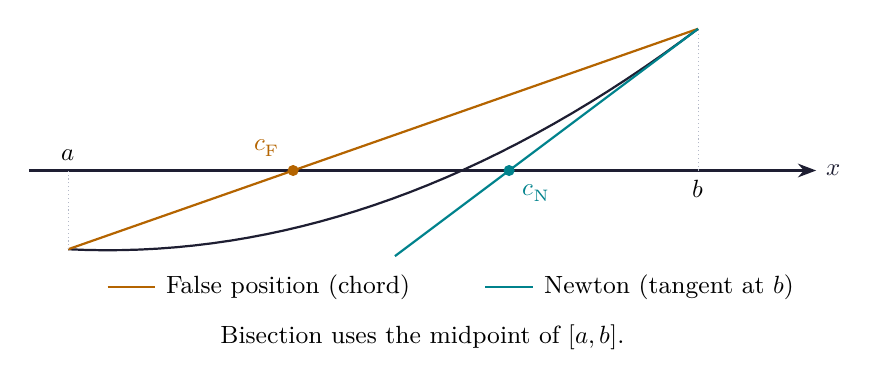
\begin{tikzpicture}[every node/.style={font=\small}]
  \draw[arrow] (-0.5,0)--(9.5,0) node[right] {$x$};
  \draw[mydark,thick,domain=0:8,samples=36] plot (\x,{0.05*(\x-5)*(\x+4)});
  \draw[myamber,thick] (0,-1)--(8,1.8);
  \draw[myteal,thick] (4.15,-1.0875)--(8,1.8);
  \draw[mgframe,densely dotted] (0,-1)--(0,0) (8,0)--(8,1.8);
  \fill[myamber] (2.857,0) circle (2pt);
  \fill[myteal] (5.6,0) circle (2pt);
  \node[above] at (0,0) {$a$};
  \node[below] at (8,0) {$b$};
  \node[above left=2pt,text=myamber] at (2.857,0) {$c_{\mathrm F}$};
  \node[below right=2pt,text=myteal] at (5.6,0) {$c_{\mathrm N}$};
  \draw[myamber,thick] (0.5,-1.48)--(1.1,-1.48);
  \node[right] at (1.12,-1.48) {False position (chord)};
  \draw[myteal,thick] (5.3,-1.48)--(5.9,-1.48);
  \node[right] at (5.92,-1.48) {Newton (tangent at $b$)};
  \node at (4.5,-2.12) {Bisection uses the midpoint of $[a,b]$.};
\end{tikzpicture}\par
\end{tcolorbox}

\newpage
\begin{center}
  {\large\bfseries\color{myred} Quick Revision --- Module 2}\\[3pt]
  {\small\color{mydark} Linear Systems and Nonlinear Equations $|$ BS-M401}
\end{center}
\noindent{\color{myred}\rule{\linewidth}{1.2pt}}\par\vspace{4pt}

\begin{tcolorbox}[formulabox, title={Key Concepts at a Glance}]
\renewcommand{\arraystretch}{1.35}
\noindent\begin{tabularx}{\linewidth}{B{4.5cm}Y}
Gauss multiplier & $m_{ik}=a_{ik}/a_{kk}$ and $R_i\leftarrow R_i-m_{ik}R_k$. \\[3pt]
LU solve & $PA=LU$ then $L\mathbf{y}=P\mathbf{b}$ and $U\mathbf{x}=\mathbf{y}$. \\[3pt]
Gauss--Seidel & Use the newly updated components in the same sweep. \\[3pt]
Bisection bound & The $k$th midpoint error is at most $(b_0-a_0)/2^k$. \\[3pt]
Newton update & $x_{k+1}=x_k-f(x_k)/f'(x_k)$. \\[3pt]
\end{tabularx}\par
\end{tcolorbox}

\begin{tcolorbox}[defbox, title={One-Line Definitions}]
\begin{itemize}[leftmargin=*, itemsep=3pt, topsep=4pt]
  \item \textbf{Pivot.} Entry used to remove other entries in a column.
  \item \textbf{Residual.} $\mathbf{b}-A\hat{\mathbf{x}}$ for a computed linear solution.
  \item \textbf{Bracket.} An interval containing a root, certified here by continuity and opposite endpoint signs.
  \item \textbf{False position.} Root estimate at the chord's intersection with the horizontal axis.
\end{itemize}
\end{tcolorbox}

\begin{tcolorbox}[exambox, title={Frequently Asked / Viva Questions}]
\begin{enumerate}[topsep=0pt, label=\textbf{Q\arabic*.}, itemsep=5pt, leftmargin=*]
  \item \Q{Why use partial pivoting?}
    It avoids zero pivots when a usable row exists and limits elimination multipliers.
  \item \Q{How do Gauss and Gauss--Jordan differ?}
    Gauss removes entries below pivots first. Gauss--Jordan also removes entries above the pivots and scales them to one.
  \item \Q{Why does LU help with many right-hand sides?}
    Keep the same factors and solve two triangular systems for each new vector.
  \item \Q{How is Gauss--Seidel different from Jacobi?}
    It uses newly computed values immediately.
  \item \Q{Name a sufficient Gauss--Seidel convergence condition.}
    Strict diagonal dominance by rows.
  \item \Q{What is checked before bisection?}
    Continuity, endpoint roots, and a sign change when neither endpoint is a root.
  \item \Q{What controls the bisection error?}
    The width of the interval before the midpoint is computed.
  \item \Q{Why can Regula-Falsi be slow?}
    One endpoint can remain fixed for many steps.
  \item \Q{What geometric line is used by Newton?}
    The tangent at the current estimate.
  \item \Q{What happens if Newton's derivative vanishes?}
    The update is undefined. Change the estimate or use a safeguarded method.
  \item \Q{What is a useful final check on a computed root?}
    Inspect the residual and a justified error or step tolerance.
\end{enumerate}
\end{tcolorbox}

\begin{tcolorbox}[tikzbox, title={Summary Comparison}]
\par\vspace{5pt}
\begingroup
\setlength{\extrarowheight}{1pt}
\noindent\begin{tabularx}{\linewidth}{|B{3.45cm}|Y|Y|}
\hline
\textbf{Method} & \textbf{What it needs} & \textbf{Main advantage} \\ \hline
Gauss or LU & Nonsingular system and usable pivots. & Direct solve with a clear substitution order. \\ \hline
Gauss--Seidel & Initial guess and convergence conditions. & Uses simple sweeps and little extra memory. \\ \hline
Bisection or false position & Continuous function with a sign-changing bracket. & Maintains a bracket under sign updates. \\ \hline
Newton--Raphson & Derivative and suitable initial estimate. & Quadratic local speed for a simple root. \\ \hline
\end{tabularx}\par
\endgroup
\end{tcolorbox}

\end{document}
